\section{Hermite Interpolation}

Osculation or Hermite Interpolation is the collocation problem extended by the requirement to match
derivatives of model function at some of the arguments.

\subsection{Solving using Divided Differences}

We can use the property that a divided difference with repeated arguments can be interpreted as a derivative:

\begin{align*}
	\underbrace{y(x_0,\ldots,x_0)}_{(n+1)}=\lim_{\xi\to x_0}\frac{y^{(n)}(\xi)}{n!}=\frac{y^{(n)}(x_0)}{n!}
\end{align*}

For example:
\makebox[\columnwidth]{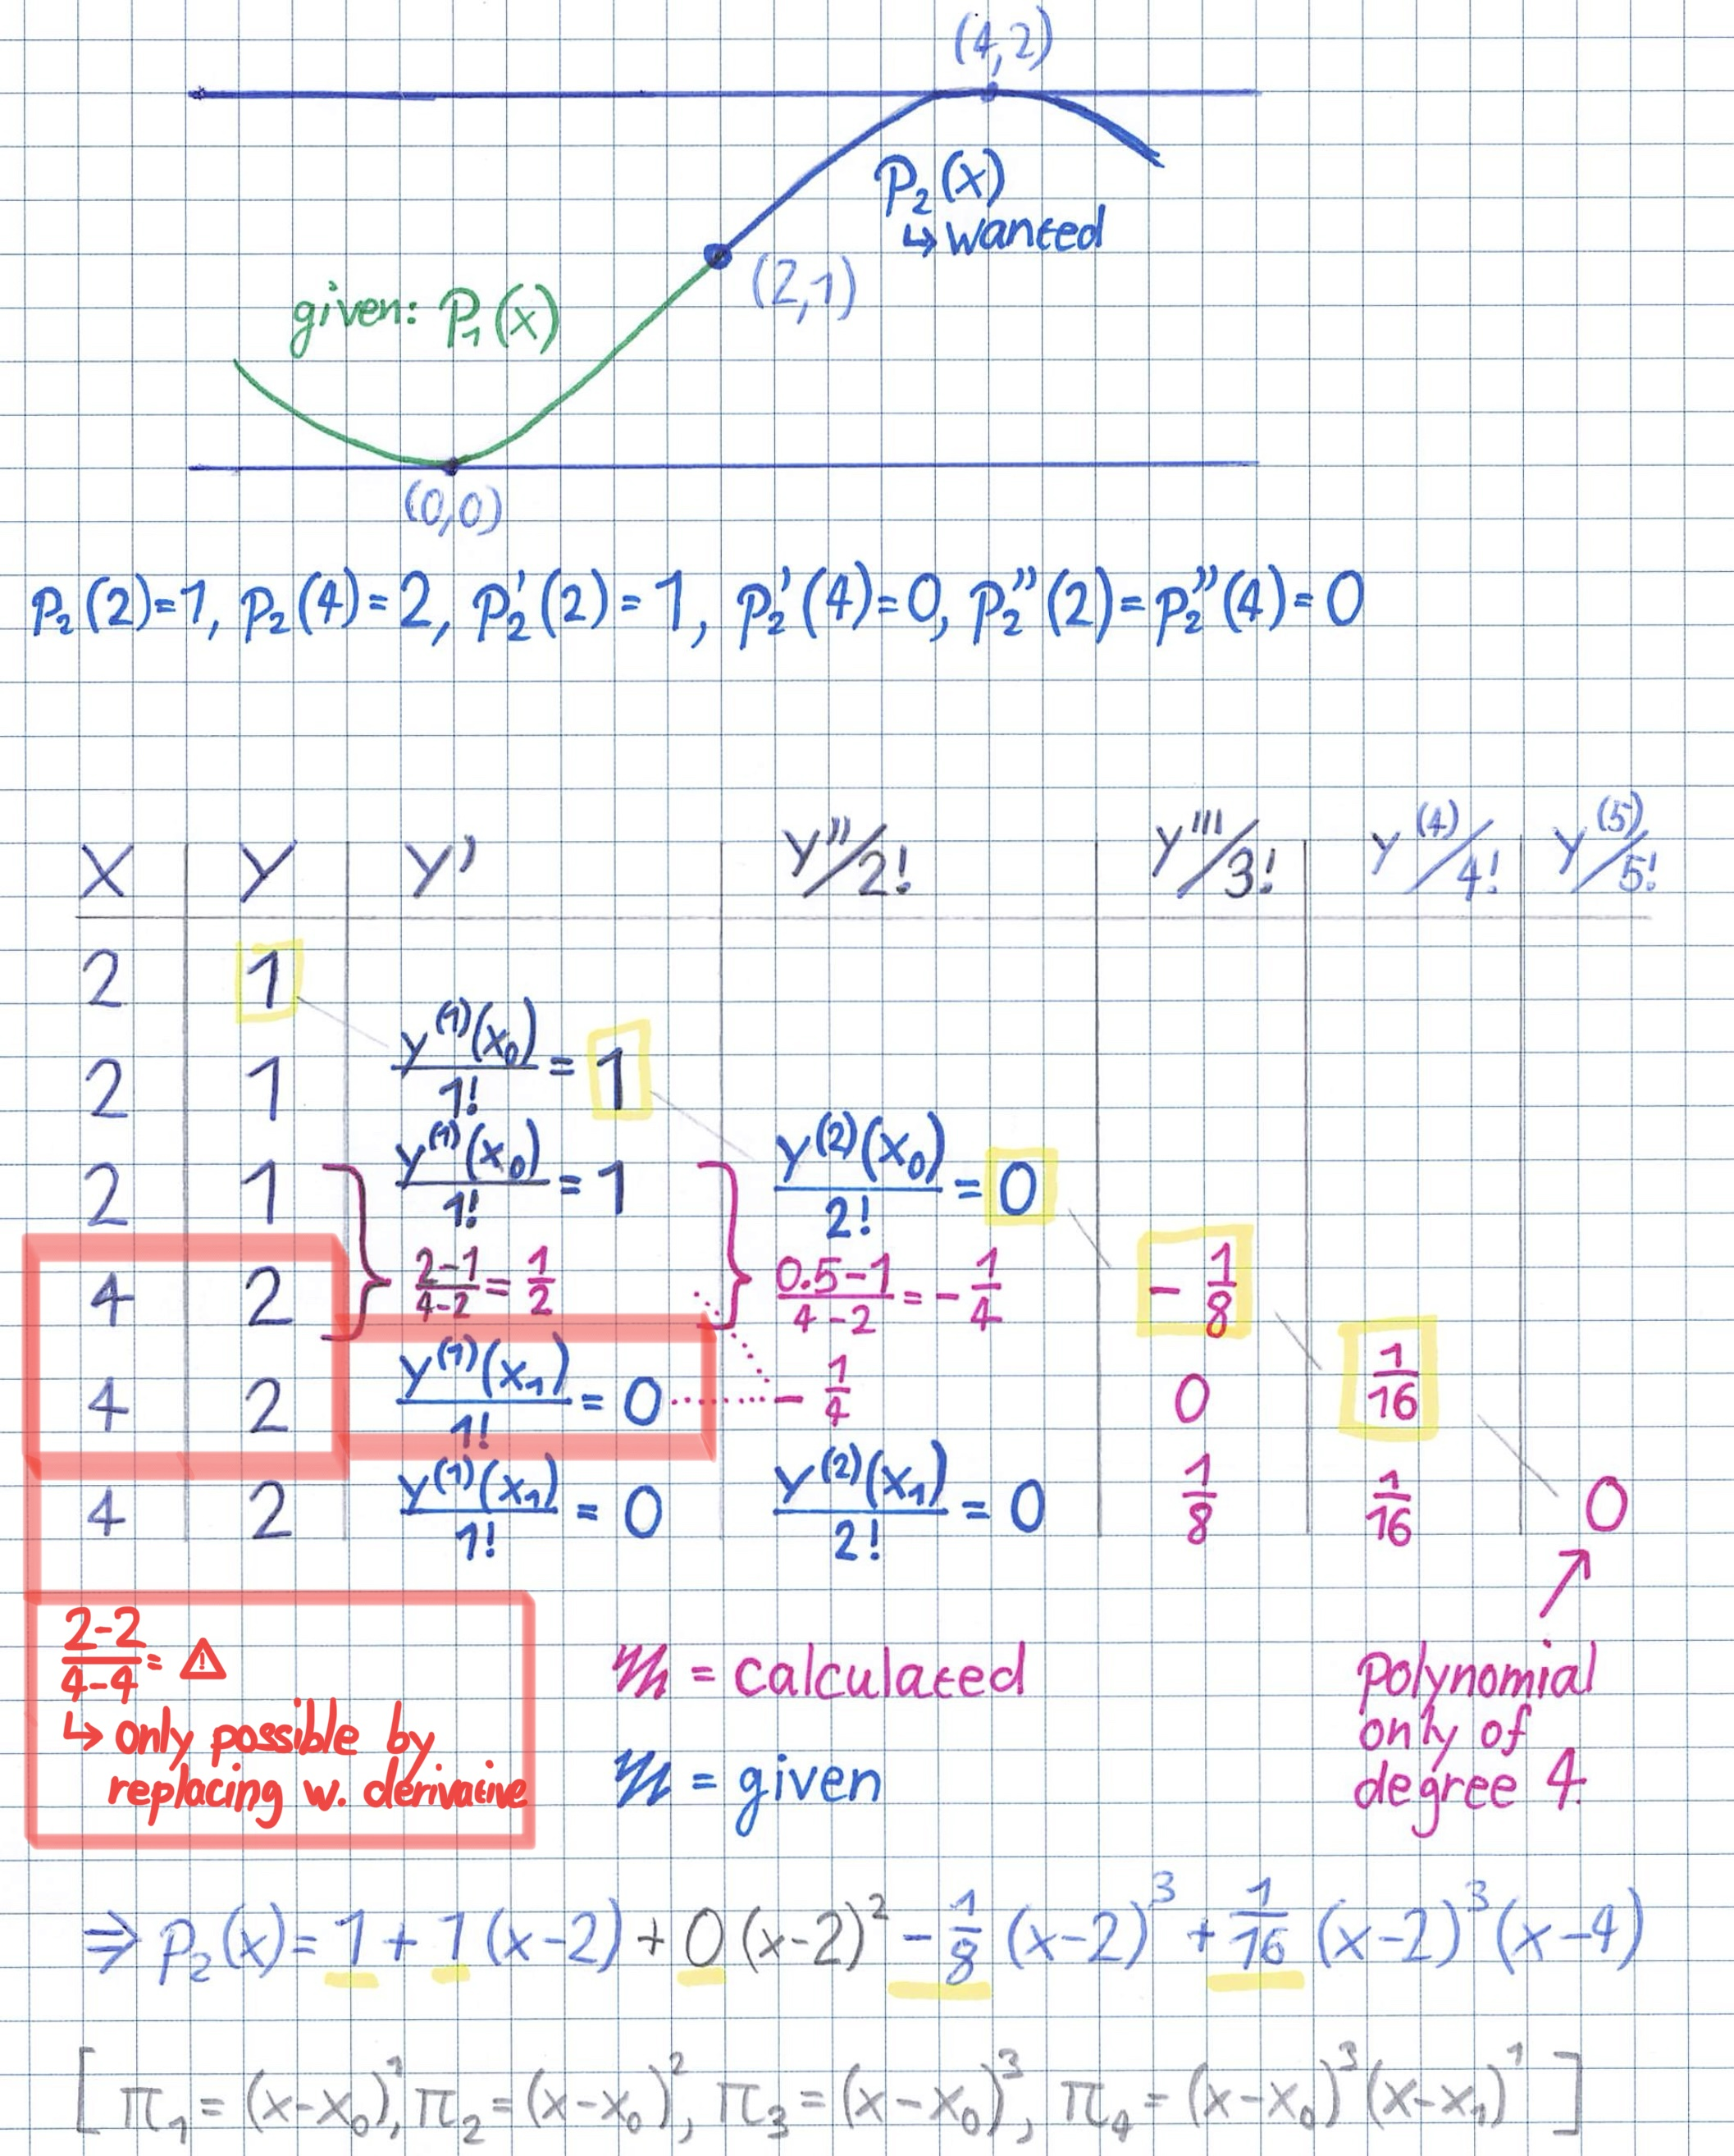
\includegraphics[width=\columnwidth]{images/hermite}}

$\pi_5$ would be $\pi_5 = (x-x_0)(x-x_0)(x-x_0)(x-x_1)(x-x_1)$ but the factor is zero, removing the need for it.

\subsection{Osculation Error Formula}

\begin{align*}
	\ & y(x)-p(x) = \frac{y^{(d)}(\xi)}{d!}(x-x_0)^{d_0}(x-x_1)^{d_1}\ldots(x-x_n)^{d_n} \\
	\ & x, \xi \in (\min x_i, \max x_i)_{i=0,1,\ldots,n}
\end{align*}

with $d$ denoting the total number of conditions and $d_i$ denoting the number of conditions for the argument $x_i\ (i=0,\ldots,n)$.
We have $d=d_0+d_1+\ldots+d_n$.

In the above example, this would be
\begin{align*}
	\frac{y^{(6)}(\xi)}{6!}(x-2)^3(x-4)^3
\end{align*}
($d$ = 6 constraints $\rightarrow$ at most degree of 5)
